\documentclass{template/nt106}

% ============================================================
% LABGUARD - ĐỀ CƯƠNG ĐỒ ÁN MÔN NT106
% Nội dung kỹ thuật được tái cấu trúc từ LABGUARD_MASTER_PLAN.pdf.
% Hình thức trình bày kế thừa template Đề_cương_KLTN_v2,
% nhưng đây KHÔNG phải đề cương KLTN.
% ============================================================

\usepackage[most]{tcolorbox}
\usepackage{listings}
\usepackage{array}
\usepackage{pifont}
\usepackage{float}
\usetikzlibrary{arrows.meta,positioning,shapes.geometric,fit,calc}

\definecolor{lgblue}{RGB}{35,89,153}
\definecolor{lglight}{RGB}{238,245,252}
\definecolor{lggreen}{RGB}{34,139,94}
\definecolor{lgorange}{RGB}{205,112,34}
\definecolor{lgred}{RGB}{183,54,54}
\definecolor{lggray}{RGB}{90,100,110}

\newtcolorbox{beginnerbox}[1][]{
  enhanced, breakable,
  colback=lglight, colframe=lgblue,
  boxrule=0.8pt, arc=2mm,
  top=1.5mm, bottom=1.5mm,
  before skip=1.2ex, after skip=1.2ex,
  title={Ghi chú nhập môn}, fonttitle=\bfseries,
  #1
}
\newtcolorbox{examplebox}[1][]{
  enhanced, breakable,
  colback=green!4, colframe=lggreen,
  boxrule=0.8pt, arc=2mm,
  top=1.5mm, bottom=1.5mm,
  before skip=1.2ex, after skip=1.2ex,
  title={Ví dụ trong LabGuard}, fonttitle=\bfseries,
  #1
}
\newtcolorbox{warningbox}[1][]{
  enhanced, breakable,
  colback=orange!5, colframe=lgorange,
  boxrule=0.8pt, arc=2mm,
  top=1.5mm, bottom=1.5mm,
  before skip=1.2ex, after skip=1.2ex,
  title={Điểm cần tránh}, fonttitle=\bfseries,
  #1
}
\newtcolorbox{vivabox}[1][]{
  enhanced, breakable,
  colback=red!3, colframe=lgred,
  boxrule=0.8pt, arc=2mm,
  top=1.5mm, bottom=1.5mm,
  before skip=1.2ex, after skip=1.2ex,
  title={Gợi ý vấn đáp cá nhân}, fonttitle=\bfseries,
  #1
}

\lstset{
  basicstyle=\ttfamily\small,
  backgroundcolor=\color{black!3},
  frame=single,
  rulecolor=\color{black!20},
  breaklines=true,
  columns=fullflexible,
  keepspaces=true,
  showstringspaces=false
}

% ---------------- Metadata ----------------
\Title{LabGuard -- Hệ thống giám sát và quản lý sự cố phòng máy}
\Title[en]{LabGuard -- Lightweight Network Monitoring and Incident Management System for Computer Labs}

% THAY THÔNG TIN NHÓM TRƯỚC KHI NỘP.
\Author{Võ Trọng Phúc}{MSSV: ........}{Lớp: ........}{SĐT: ........}
\Author{Thành viên 2}{MSSV: ........}{Lớp: ........}{SĐT: ........}
\Author{Thành viên 3}{MSSV: ........}{Lớp: ........}{SĐT: ........}
\Advisor{........................................................}
\Faculty{Khoa Mạng máy tính và Truyền thông}
\ThesisFromDate{09/2026}
\ThesisToDate{10/2026}

\renewcommand{\figureautorefname}{Hình}
\renewcommand{\tableautorefname}{Bảng}
\renewcommand{\sectionautorefname}{Mục}
\renewcommand{\subsectionautorefname}{Mục}
\hypersetup{colorlinks=true,linkcolor=blue,citecolor=blue,urlcolor=blue,pdftitle={LabGuard -- Hệ thống giám sát và quản lý sự cố phòng máy},pdfauthor={Võ Trọng Phúc}}

\begin{document}
\printinfo

\begin{center}
\textbf{Biên soạn:} Võ Trọng Phúc\\
\textit{Tài liệu này trình bày lại Project Blueprint theo phong cách đề cương học thuật của UIT. Đây là đề cương đồ án môn NT106, không phải khóa luận tốt nghiệp.}
\end{center}

\vspace*{1ex}

\section{Tổng quan đề tài:}
\label{sec:tong-quan-de-tai}
% ============================================================
% 1. TỔNG QUAN ĐỀ TÀI
% ============================================================

\subsection*{1. Bối cảnh và vấn đề thực tế}

Trong một phòng máy hoặc phòng thực hành, người quản trị thường phải theo dõi đồng thời nhiều máy tính. Một máy có thể vẫn đang bật nhưng dịch vụ quan trọng đã ngừng phản hồi; một máy khác có thể mất kết nối mạng; một máy khác lại có mức sử dụng CPU hoặc RAM tăng bất thường. Nếu chỉ chờ người dùng báo lỗi rồi mới đến từng máy kiểm tra, thời gian phát hiện và xử lý sự cố sẽ kéo dài, đồng thời khó biết ai đang phụ trách sự cố nào.

Đồ án \textbf{LabGuard} được đề xuất như một hệ thống giám sát và quản lý sự cố nhẹ cho phòng máy, kế thừa thiết kế từ tài liệu Master Plan \cite{labguard2026}, bám sát chuẩn đầu ra kiến thức của môn học Lập trình mạng căn bản (NT106) tại UIT \cite{uit_nt106_2022}. Mỗi máy cần giám sát chạy một chương trình nhỏ gọi là \textbf{Agent}. Agent gửi trạng thái máy về máy chủ trung tâm. Máy chủ không chỉ lưu dữ liệu mà còn đánh giá các điều kiện bất thường, tạo \textbf{Incident} (phiếu sự cố), ghi lại quá trình xử lý và đồng bộ trạng thái cho nhiều quản trị viên cùng lúc.

\begin{beginnerbox}
\textbf{Hiểu nhanh 5 từ khóa trước khi đọc tiếp:}
\begin{itemize}
    \item \textbf{Agent}: chương trình chạy trên máy được giám sát, có nhiệm vụ thu thập trạng thái và gửi về server.
    \item \textbf{Telemetry}: dữ liệu trạng thái gửi từ xa, ví dụ CPU, RAM, uptime, trạng thái cổng dịch vụ.
    \item \textbf{Heartbeat}: gói ``nhịp tim'' gửi định kỳ để server biết Agent vẫn còn hoạt động.
    \item \textbf{Incident}: bản ghi một sự cố cần được theo dõi từ lúc phát hiện đến lúc xử lý xong.
    \item \textbf{Admin Dashboard}: ứng dụng quản trị dùng để xem máy, xem sự cố và thao tác ACK/START/RESOLVE.
\end{itemize}
\end{beginnerbox}

\subsection*{2. Vấn đề của cách theo dõi đơn giản}

Một chương trình chỉ hiển thị CPU/RAM trên dashboard chưa đủ để trở thành một hệ thống xử lý sự cố. Vấn đề thực tế không chỉ là ``máy đang có CPU bao nhiêu phần trăm'', mà còn là:
\begin{itemize}
    \item máy nào đang mất liên lạc và mất từ khi nào;
    \item dịch vụ nào trên máy không còn phản hồi;
    \item một cảnh báo đã tồn tại từ trước hay vừa mới phát sinh;
    \item ai đang nhận xử lý sự cố;
    \item trạng thái đã phục hồi hay chưa;
    \item sau khi server hoặc ứng dụng khởi động lại, lịch sử sự cố có còn hay không;
    \item nếu hai quản trị viên thao tác cùng lúc thì hệ thống phải xử lý xung đột thế nào;
    \item nếu mạng chập chờn, dữ liệu bị gửi trùng hoặc mất kết nối, hệ thống có tạo cảnh báo sai hoặc nhân đôi Incident hay không.
\end{itemize}

Vì vậy, giá trị cốt lõi của LabGuard nằm ở \textbf{vòng đời xử lý sự cố, tính đúng đắn khi mạng không ổn định và khả năng phối hợp nhiều quản trị viên}, chứ không nằm ở việc vẽ nhiều biểu đồ.

\subsection*{3. Hệ thống đề xuất}

Phiên bản tối thiểu (MVP) của LabGuard gồm ba nhóm thành phần: \textbf{Agent}, \textbf{Central Server} và \textbf{Admin Client}. Central Server giữ trạng thái nghiệp vụ chính và làm việc với SQL Server. Sau khi MVP ổn định, hệ thống có thể mở rộng thêm Gateway và hai Collector để minh họa multi-server và load balancing.

\begin{figure}[!ht]
    \centering
    \begin{tikzpicture}[
        node distance=1.6cm and 1.8cm,
        box/.style={draw=lgblue, rounded corners=2mm, fill=lglight, minimum width=3.0cm, minimum height=1cm, align=center},
        db/.style={cylinder, shape border rotate=90, aspect=0.25, draw=lgblue, fill=blue!5, minimum height=1.3cm, minimum width=2.0cm, align=center},
        arr/.style={-{Latex[length=2.5mm]}, thick, draw=lgblue}
    ]
        \node[box] (a1) {Agent PC-01};
        \node[box, below=0.6cm of a1] (a2) {Agent PC-02};
        \node[box, below=0.6cm of a2] (an) {Agent PC-n};
        \node[box, right=of a2] (central) {Central Server\\(Cơ chế Incident)};
        \node[db, right=of central] (db) {SQL Server};
        \node[box, above=1.2cm of db] (admin1) {Admin Client A};
        \node[box, below=1.2cm of db] (admin2) {Admin Client B};
        \draw[arr] (a1.east) -- (central.west);
        \draw[arr] (a2.east) -- (central.west);
        \draw[arr] (an.east) -- (central.west);
        \draw[arr] (central.east) -- (db.west);
        \draw[arr,<->] (central.north east) -- (admin1.west);
        \draw[arr,<->] (central.south east) -- (admin2.west);
    \end{tikzpicture}
    \caption{Kiến trúc MVP của LabGuard.}
    \label{fig:labguard-mvp}
\end{figure}

\begin{examplebox}
Một kịch bản điển hình:
\begin{enumerate}
    \item PC07 đang gửi heartbeat bình thường.
    \item Agent trên PC07 không còn kết nối được tới cổng dịch vụ 8080 trong nhiều lần kiểm tra liên tiếp.
    \item Central Server tạo một Incident loại \texttt{SERVICE\_DOWN}.
    \item Admin A bấm \texttt{ACKNOWLEDGE}, sau đó \texttt{START} để nhận xử lý.
    \item Dịch vụ hoạt động trở lại, Agent báo trạng thái phục hồi.
    \item Incident chuyển sang \texttt{RECOVERED}; Admin xác nhận và chuyển sang \texttt{RESOLVED}.
    \item Toàn bộ lịch sử vẫn được lưu trong cơ sở dữ liệu.
\end{enumerate}
\end{examplebox}

\subsection*{4. Đối tượng sử dụng và phạm vi sử dụng}

Đối tượng chính của hệ thống là quản trị viên phòng máy, người trực vận hành và người xem read-only như giảng viên khi demo. MVP chỉ xét một tổ chức và một phòng lab mặc định; \texttt{LabCode} chỉ dùng như nhãn lọc. Đồ án không đặt mục tiêu xây dựng nền tảng multi-tenant hoặc hệ thống phân quyền phức tạp theo từng phòng.

\begin{table}[!ht]
\centering
\caption{Nhóm người dùng chính của LabGuard.}
\label{tab:personas}
\begin{tabularx}{\textwidth}{>{\bfseries}p{3.2cm} X X}
\toprule
Đối tượng & Nhu cầu chính & Luồng sử dụng điển hình \\
\midrule
Admin phòng máy & Quan sát toàn phòng, phân công xử lý, cấp tài khoản & Dashboard $\rightarrow$ Assign $\rightarrow$ History \\
Operator trực & Biết máy nào cần xử lý và tránh trùng công việc & Lab View $\rightarrow$ ACK/START $\rightarrow$ Resolve \\
Viewer / giảng viên & Xem trạng thái nhưng không thay đổi dữ liệu & Devices / Incidents / Health ở chế độ read-only \\
\bottomrule
\end{tabularx}
\end{table}

\subsection*{5. Use case chính}

\begin{table}[!ht]
\centering
\caption{Các use case cốt lõi của LabGuard.}
\label{tab:usecases}
\small
\begin{tabularx}{\textwidth}{p{1.2cm} X X}
\toprule
\textbf{UC} & \textbf{Luồng chính} & \textbf{Trường hợp lỗi cần xử lý} \\
\midrule
UC01 & Seed Admin $\rightarrow$ login; Mở rộng: invite $\rightarrow$ signup $\rightarrow$ login & Invite hết hạn hoặc đã dùng phải bị từ chối \\
UC02 & Agent enroll $\rightarrow$ TLS/auth $\rightarrow$ metrics/heartbeat & Token/certificate sai $\rightarrow$ Blocked; mạng lỗi $\rightarrow$ Backoff \\
UC03 & Lab View $\rightarrow$ Device Detail & Dữ liệu cũ phải hiển thị rõ là stale/Unknown \\
UC04 & Nhiều mẫu bất thường $\rightarrow$ mở/cập nhật Incident & Replay hoặc null không được tạo spam Incident \\
UC05 & ACK $\rightarrow$ START $\rightarrow$ RECOVERED $\rightarrow$ RESOLVE & Hai Admin thao tác đồng thời phải phát hiện conflict \\
UC06 & History/report theo khoảng thời gian & Viewer không có quyền mutation \\
UC07 & Reconnect $\rightarrow$ tạo session generation mới & Session cũ và batch trùng phải bị loại \\
UC08 (P1) & Gateway chọn Collector khỏe và ít kết nối hơn & Collector chết $\rightarrow$ Agent reconnect sang node khác \\
\bottomrule
\end{tabularx}
\end{table}

\subsection*{6. Điểm khác biệt của đồ án}

Theo Master Plan nguồn, LabGuard được định hướng như một \textbf{sản phẩm môn Lập trình mạng} thay vì một dashboard quản lý dữ liệu. Trọng tâm thiết kế là TCP/TLS, nhiều client, xử lý kết nối mất/khôi phục, giao thức tầng ứng dụng có framing, đồng bộ trạng thái nhiều Admin, lưu bền dữ liệu, kiểm thử lỗi mạng và -- nếu MVP đạt yêu cầu -- mở rộng multi-server/load balancing.

\begin{warningbox}
Tài liệu nguồn chưa xác minh rubric chính thức của lớp và chưa chạy sản phẩm thực tế. Vì vậy, mọi ngưỡng như ``50 Agent'', ``offline 20 giây'' hoặc kế hoạch P1 chỉ là \textbf{mục tiêu thiết kế}, không phải kết quả đã đo hay cam kết điểm số.
\end{warningbox}


\section{Mục tiêu của đề tài:}
\label{sec:muc-tieu-de-tai}
% ============================================================
% 2. MỤC TIÊU ĐỀ TÀI
% ============================================================

\subsection*{a) Mục tiêu tổng quát}

Xây dựng một hệ thống \textbf{LabGuard} có khả năng giám sát nhiều máy tính trong phòng lab thông qua kết nối mạng, phát hiện một số tình trạng bất thường cơ bản, tổ chức vòng đời xử lý sự cố và hỗ trợ nhiều quản trị viên phối hợp theo thời gian thực. Hệ thống được triển khai chủ yếu bằng C\#, WinForms, TCP/TLS và SQL Server, qua đó thể hiện các kiến thức cốt lõi của môn NT106 như socket, I/O mạng, multi-client, concurrency, cơ sở dữ liệu, bảo mật kết nối, triển khai LAN và kiểm thử lỗi mạng.

\subsection*{b) Mục tiêu cụ thể}

\begin{itemize}
    \item \textbf{Xây dựng Agent Windows}: thu thập CPU, RAM vật lý, NIC, uptime; gửi heartbeat và telemetry; kiểm tra một số cổng TCP cục bộ; tự reconnect khi mạng lỗi.

    \item \textbf{Xây dựng Central Server}: tiếp nhận nhiều Agent đồng thời, xác thực phiên, xử lý message framing, lưu dữ liệu, quản lý trạng thái online/offline và thực thi các rule phát hiện sự cố.

    \item \textbf{Xây dựng Incident Engine}: hỗ trợ ít nhất các nhóm sự cố như mất heartbeat, CPU cao, RAM cao và service/port không phản hồi; chống tạo trùng Incident và lưu lịch sử thay đổi trạng thái.

    \item \textbf{Xây dựng Admin Client bằng WinForms}: login, Dashboard, Lab View, Device Detail, Incident List/Detail, History/Report và Server Health; hai Admin có thể quan sát trạng thái realtime.

    \item \textbf{Thiết kế giao thức tầng ứng dụng trên TCP}: dùng length-prefix để xác định biên message, JSON UTF-8 làm payload và quy định rõ các trường version, messageType, requestId, deviceId, timestamp và payload.

    \item \textbf{Áp dụng bảo mật phù hợp}: dùng TLS cho dữ liệu truyền trên mạng; mật khẩu được băm bằng KDF có salt; quyền thao tác được kiểm tra ở phía server; không tự thiết kế thuật toán mã hóa riêng.

    \item \textbf{Kiểm thử multi-client và lỗi mạng}: sử dụng Agent Simulator tạo 10/20/50 kết nối độc lập; kiểm thử disconnect, reconnect, malformed packet, duplicate packet, server restart và reconnect storm.

    \item \textbf{Triển khai LAN thực tế}: ít nhất 2--3 laptop vật lý, kết hợp simulated agents để chứng minh sản phẩm không chỉ chạy localhost.

    \item \textbf{Mở rộng có điều kiện P1}: sau khi MVP ổn định, xây Gateway và hai Collector để minh họa health check, least-connections, failover có gián đoạn và load balancing ở mức phù hợp đồ án môn học.

    \item \textbf{Chuẩn bị vấn đáp cá nhân}: mỗi thành viên sở hữu phần kỹ thuật riêng, có task, test, bằng chứng và bộ câu hỏi vấn đáp bám đúng code/module mình thực hiện.
\end{itemize}

\begin{beginnerbox}
\textbf{MVP là gì?} MVP (Minimum Viable Product) là phiên bản nhỏ nhất nhưng đã chạy được một luồng sản phẩm hoàn chỉnh. Với LabGuard, MVP không có nghĩa là ``demo giả''. MVP phải có Agent thật $\rightarrow$ TCP/TLS $\rightarrow$ Central $\rightarrow$ SQL $\rightarrow$ Admin, có Incident và có kiểm thử LAN. Gateway/Collector là phần nâng cao, không được làm trước khi MVP ổn định.
\end{beginnerbox}


\section{Phương pháp thực hiện:}
\label{sec:phuong-phap-thuc-hien}
% ============================================================
% 3. PHƯƠNG PHÁP THỰC HIỆN
% ============================================================

\begin{enumerate}
    \item \textbf{Khảo sát yêu cầu và đóng băng phạm vi MVP}

    Nhóm xác định rõ các chức năng bắt buộc, các chức năng nâng cao và các nội dung không làm. Các quyết định kỹ thuật được ghi lại trước khi triển khai để tránh thay đổi protocol/schema tùy tiện giữa dự án. Phần P1 multi-server chỉ được bắt đầu sau khi MVP qua gate cuối tuần 3.

    \item \textbf{Thiết kế kiến trúc theo từng mức độ phức tạp}

    Giai đoạn đầu dùng kiến trúc đơn giản: nhiều Agent kết nối trực tiếp đến Central Server; Admin Client cũng kết nối đến Central; chỉ Central truy cập SQL Server. Khi core ổn định, P1 bổ sung Gateway và hai Collector ở lớp Agent-facing nhưng vẫn giữ Central là nơi duy nhất quyết định nghiệp vụ Incident.

    \begin{beginnerbox}
    \textbf{Tại sao không làm multi-server ngay từ đầu?} Nếu ngay tuần đầu đã thêm Gateway, hai Collector, failover và load balancing, nhóm sẽ phải debug nhiều tầng cùng lúc. Khi một message không tới DB, rất khó biết lỗi nằm ở Agent, Gateway, Collector hay Central. Vì vậy Master Plan yêu cầu chứng minh một luồng end-to-end đơn giản trước, sau đó mới thêm phân tán.
    \end{beginnerbox}

    \item \textbf{Thiết kế giao thức TCP có framing}

    TCP \cite{rfc9293} được chọn cho các kết nối chính vì ứng dụng cần truyền dữ liệu có thứ tự và tin cậy. Tuy nhiên TCP là một \textbf{byte stream}; một lần gọi \texttt{ReadAsync} không đồng nghĩa với một message hoàn chỉnh. Do đó LabGuard sử dụng \textbf{length-prefix framing}: trước mỗi JSON envelope UTF-8 có đúng 4 byte biểu diễn độ dài $N$ (kiểu \texttt{uint32} theo trật tự mạng Big-Endian). Giá trị $N$ chỉ tính riêng kích thước payload JSON, không tính 4 byte header prefix.

    \begin{examplebox}
    Giả sử cần gửi chuỗi JSON dài 120 byte. Bên gửi truyền tổng cộng 124 byte trên wire dạng \texttt{[00 00 00 78] [120 byte JSON UTF-8]} (với \texttt{0x00000078 = 120}). Phía nhận trước hết đọc đủ 4 byte để biết message dài bao nhiêu, kiểm tra giới hạn an toàn, rồi tiếp tục đọc cho tới khi đủ 120 byte. Nếu hệ điều hành trả về 30 byte ở lần đọc đầu và 90 byte ở lần sau (hiện tượng \textit{partial read}), bộ giải mã \texttt{FrameCodec} vẫn gom đủ đúng 120 byte trước khi chuyển sang tầng phân tích JSON. Về lý thuyết, JSON hợp lệ (RFC 8259 \cite{rfc8259}) bắt buộc escape ký tự xuống dòng thành \texttt{\textbackslash n} nên giao thức phân tách bằng newline trên JSON đơn dòng vẫn có thể dùng được; tuy nhiên LabGuard chọn length-prefix vì nó cung cấp contract nhị phân tường minh, biết trước kích thước để cấp phát bộ đệm một lần và kiểm soát parser chặt chẽ.
    \end{examplebox}

    Kích thước frame được giới hạn ở mức thiết kế $N \leq 256$ KiB để ngăn ngừa tấn công làm tràn bộ nhớ RAM (OutOfMemory DoS). Envelope chuẩn hóa gồm \texttt{version}, \texttt{messageType}, \texttt{requestId}, \texttt{deviceId}, \texttt{sentAtUtc} và \texttt{payload} (trong đó cờ \texttt{isReplay} được đặt bên trong payload của telemetry và service status).

    \item \textbf{Xây dựng Agent và cơ chế liveness}

    Agent thu thập CPU host, RAM vật lý, NIC, uptime và kết quả kiểm tra cổng TCP cục bộ. Heartbeat được gửi định kỳ mỗi 5 giây để Central Server đánh giá liveness. Nếu mất kết nối, Agent chuyển sang chế độ lùi lũy tiến ngẫu nhiên (\textit{exponential backoff with jitter}) rồi reconnect thay vì lặp lại kết nối liên tục làm quá tải server.

    \begin{beginnerbox}
    \textbf{Heartbeat khác ``TCP Connected'' thế nào?} Thuộc tính \texttt{Socket.Connected} trong .NET \cite{mslearn_sockets} chỉ phản ánh trạng thái của kết nối tại thời điểm của thao tác I/O gần nhất; nếu máy client bị mất nguồn hoặc đứt cáp đột ngột, server vẫn thấy \texttt{Connected == true}. Heartbeat là bằng chứng sống ở tầng ứng dụng: nếu quá 20 giây kể từ heartbeat hợp lệ gần nhất (tính theo đồng hồ đơn điệu phía server để tránh sai lệch NTP), server chủ động đánh dấu thiết bị là \texttt{OFFLINE} và đóng socket.
    \end{beginnerbox}

    \item \textbf{Xây dựng Central Server, rule engine và Incident Engine}

    Central xử lý nhiều socket đồng thời bằng mô hình bất đồng bộ trên ThreadPool \cite{mslearn_sockets}. Theo tài liệu chính thức từ Microsoft \cite{mslearn_networkstream}, lớp \texttt{NetworkStream} chỉ bảo đảm an toàn cho 1 thao tác đọc và 1 thao tác ghi đồng thời; việc nhiều tác vụ cùng gọi ghi đồng thời không được hỗ trợ an toàn nếu không tự đồng bộ. Do đó LabGuard sử dụng hàng đợi gửi đơn luồng (\texttt{System.Threading.Channels} \cite{mslearn_channels}) cho từng kết nối. Central xác thực Agent/Admin, nhận telemetry, khử trùng lặp (\textit{deduplication}) batch dựa trên bộ ba \texttt{DeviceId + BootId + BatchId}, cập nhật trạng thái thiết bị, đánh giá rule và lưu dữ liệu. Incident được tạo theo khóa logic để một điều kiện bất thường chỉ có duy nhất một Incident active thay vì mỗi chu kỳ gửi dữ liệu lại tạo thêm một ticket rác.

    Rule không chỉ dựa vào một ngưỡng tức thời mà áp dụng \textbf{streak} (số mẫu vi phạm liên tiếp) và \textbf{hysteresis} (vùng trễ giữa ngưỡng mở và ngưỡng phục hồi) để tránh hiện tượng cảnh báo nhấp nháy (\textit{alert flapping}) khi giá trị dao động sát ngưỡng.

    \begin{examplebox}
    Với CPU: mở cảnh báo \texttt{HIGH\_CPU} khi CPU $\geq 90\%$ trong 3 mẫu liên tiếp (chu kỳ lấy mẫu 5 giây, khoảng thời gian từ mẫu 1 đến mẫu 3 là 10 giây); chỉ coi là phục hồi khi CPU $\leq 75\%$ trong 3 mẫu liên tiếp. Khoảng cách trễ 15\% giúp hệ thống lọc nhiễu hiệu quả khi CPU dao động quanh ngưỡng 90\%.
    \end{examplebox}

    \item \textbf{Thiết kế cơ sở dữ liệu và tính nhất quán}

    SQL Server 2022 Express là cơ sở dữ liệu baseline duy nhất của đề tài; chỉ Central Server truy cập trực tiếp DB. Dữ liệu gồm users, devices, telemetry, services, incidents, incident history, collector health và audit log. Incident cần transaction và \texttt{rowversion} để xử lý trường hợp hai Admin cùng thao tác một bản ghi.

    \begin{beginnerbox}
    \textbf{Race condition và rowversion:} Giả sử Incident đang OPEN. Admin A và B cùng đọc trạng thái rồi gần như đồng thời bấm ACK. Trong SQL Server, cột kiểm soát tương tranh phải được khai báo bằng kiểu chuyên biệt \texttt{rowversion} \cite{mslearn_rowversion}, được client xử lý như token nhị phân 8 byte opaque (không phải ngày giờ); một cột \texttt{binary(8)} thông thường không có hành vi tự động cập nhật tương đương. Mỗi khi dòng dữ liệu bị sửa đổi, \texttt{rowversion} tự động đổi sang số mới. Server thực hiện câu lệnh có điều kiện \texttt{WHERE rowversion = @oldVersion}; thao tác đến sau sẽ nhận 0 dòng bị ảnh hưởng và server trả mã \texttt{CONFLICT}.
    \end{beginnerbox}

    \item \textbf{Xây dựng Admin Client và đồng bộ realtime}

    Admin Client hiển thị snapshot ban đầu rồi nhận các delta/event mới. Khi reconnect, client cần đồng bộ lại state thay vì giả định cache cũ vẫn đúng. UI không được block trong lúc chờ network; dữ liệu cập nhật từ background task phải được marshal về UI thread bằng \texttt{Control.Invoke}, \texttt{BeginInvoke} hoặc \texttt{InvokeAsync} \cite{mslearn_winforms_threadsafe} tùy target framework (.NET 9+ hỗ trợ InvokeAsync). Việc ẩn hoặc làm mờ nút trên UI chỉ là cải thiện trải nghiệm người dùng (UX), không thay thế bảo mật; Central Server bắt buộc phải kiểm tra quyền (server-side authorization) đối với mọi lệnh nhận được trước khi thực thi.

    \item \textbf{Bảo mật ở mức phù hợp đồ án}

    TLS/SslStream \cite{rfc8446,mslearn_sslstream} được áp dụng từ đầu cho kết nối. Về lưu trữ mật khẩu: OWASP recommends Argon2id for new systems generally. If FIPS-140 compliance is required, OWASP recommends PBKDF2-HMAC-SHA256 with a work factor of 600,000 or more. LabGuard deliberately chooses PBKDF2 for BCL availability and course-scope simplicity; 600,000 is therefore the project baseline referenced from OWASP and must still be measured on the actual lab hardware \cite{owasp_password_storage}. Salt 16 byte và key 32 byte là tham số thiết kế; lưu algorithm và work factor để hỗ trợ nâng cấp; so sánh hash thời gian hằng số qua \texttt{FixedTimeEquals}; session gắn socket và server kiểm tra authorization cho mutation. Đồ án không tự chế thuật toán mã hóa.

    \begin{beginnerbox}
    \textbf{Phân biệt 4 khái niệm bảo mật:} \textbf{Encryption} (bảo vệ tính bí mật trên đường truyền); \textbf{Hashing} (băm một chiều mật khẩu kèm salt ngẫu nhiên); \textbf{Authentication} (xác định danh tính người dùng/máy trạm); \textbf{Authorization} (kiểm tra quyền hạn thực thi phía server).
    \end{beginnerbox}

    \item \textbf{Kiểm thử tăng dần và failure injection}

    Nhóm kiểm thử parser, threshold, state transition, DB transaction, multi-client, reconnect và các failure case trước khi polish UI. Agent Simulator tạo nhiều socket độc lập để kiểm tra tải mà không cần 20--50 máy thật. Mỗi test phải có setup, action, expected result và evidence/log.

    \item \textbf{Triển khai, demo và audit}

    MVP dự kiến thử nghiệm và demo trên 3 máy tính xách tay: máy 1 chạy Central và SQL, máy 2 chạy Agent kèm Simulator, máy 3 chạy Admin cùng Agent. Triển khai Internet chỉ được tính hoàn thành khi có bằng chứng sơ đồ mạng và route hợp lệ. ChatGPT Work đóng vai trò auditor độc lập: rà soát tính nhất quán, rủi ro, phạm vi và bằng chứng thực nghiệm; không coi kết quả thẩm định tài liệu là bằng chứng sản phẩm chạy thực tế.
\end{enumerate}


\section{Các nội dung chính và giới hạn của đề tài:}
\label{sec:noi-dung}
% ============================================================
% 4. CÁC NỘI DUNG CHÍNH VÀ GIỚI HẠN
% ============================================================

\subsection{Nội dung 1: Xác lập yêu cầu, phạm vi và contract kỹ thuật}

\begin{itemize}
    \item \textbf{Mục tiêu:} thống nhất giữa ba thành viên về chức năng P0/P1, message envelope, schema chính, ownership và tiêu chí DONE trước khi code tăng nhanh.
    \item \textbf{Phương pháp thực hiện:} tạo fixtures mẫu cho protocol, migration ban đầu, mock DTO cho UI, thống nhất quy tắc branch/PR và ghi các thay đổi lớn bằng decision record.
\end{itemize}

\begin{table}[!ht]
\centering
\caption{Phạm vi ưu tiên theo Master Plan.}
\label{tab:scope-priority}
\small
\begin{tabularx}{\textwidth}{p{1.2cm} X X}
\toprule
\textbf{Mức} & \textbf{Nội dung} & \textbf{Ý nghĩa} \\
\midrule
P0 & Agent Windows, telemetry, heartbeat, local TCP probe, reconnect; Central nhiều Agent; Incident; DB; WinForms; auth/roles; TLS; simulator; LAN & Bắt buộc để có một sản phẩm NT106 hoàn chỉnh \\
P1 & Gateway least-connections, 2 Collector, readiness/failover/fencing & Chỉ làm sau MVP gate; dùng để tăng chiều sâu multi-server \\
P2 & Manual probe allowlist nâng cao, threshold versioning, minute aggregates, latency rule, weighted LB & Stretch feature sau release candidate nếu còn thời gian \\
P3 & Agent Linux, multi-lab phức tạp, Central HA, AI/anomaly & Hướng tương lai, không nằm trong cam kết 5 tuần \\
Không làm & Remote desktop/shell, restart service từ xa, đọc file/process nhạy cảm, Kubernetes, Redis/Kafka, web frontend lớn & Tránh lệch trọng tâm và scope explosion \\
\bottomrule
\end{tabularx}
\end{table}

\subsection{Nội dung 2: Agent, telemetry và kết nối mạng phía client}

\begin{itemize}
    \item \textbf{Mục tiêu:} mỗi Agent có thể kết nối an toàn đến server, gửi trạng thái định kỳ, phát hiện lỗi cục bộ và tự phục hồi kết nối khi mạng gián đoạn.
    \item \textbf{Dữ liệu P0:} CPU host, RAM vật lý, NIC, uptime và kết quả TCP service probe trong allowlist tối đa 5 mục ở bản MVP.
    \item \textbf{Kỹ thuật chính:} TcpClient/SslStream, writer queue, heartbeat, batching, reconnect backoff, local log và Agent Simulator.
\end{itemize}

\begin{examplebox}
Agent Simulator không phải ``vẽ giả 50 máy'' trên UI. Mỗi simulated Agent phải có \textbf{socket riêng, DeviceId riêng, heartbeat riêng và state riêng}. Khi đó server thực sự phải xử lý 10/20/50 client concurrent, phù hợp để kiểm thử multi-client mà không cần 50 máy vật lý.
\end{examplebox}

\subsection{Nội dung 3: Central Server, liveness và rule engine}

Central là thành phần nghiệp vụ trung tâm của MVP. Server nhận kết nối TLS, parse frame có giới hạn, bind session với identity, cập nhật device registry, commit telemetry và gửi ACK phù hợp. Liveness được đánh giá dựa trên heartbeat/deadline đo bằng monotonic clock của server chứ không chỉ dựa vào trạng thái socket.

Bốn nhóm rule P0 dự kiến:
\begin{enumerate}
    \item \texttt{DEVICE\_OFFLINE}: không nhận heartbeat hợp lệ trong khoảng thời gian $> 20$ giây (đo bằng \texttt{Stopwatch} / monotonic clock tại server, độc lập với wall-clock client);
    \item \texttt{HIGH\_CPU}: CPU vượt ngưỡng $\ge 90\%$ trong 3 sample liên tiếp (chu kỳ lấy mẫu 5 giây, khoảng thời gian từ mẫu 1 đến mẫu 3 là 10 giây); phục hồi khi CPU $\le 75\%$ trong 3 sample liên tiếp (dải trễ hysteresis 15\% chống rung lắc trạng thái);
    \item \texttt{HIGH\_MEMORY}: RAM vượt ngưỡng quy định trong 3 sample liên tiếp (chu kỳ 5 giây);
    \item \texttt{SERVICE\_DOWN}: TCP probe tới cổng dịch vụ thất bại trong 2 lần thăm dò liên tiếp (timeout 2 giây/lần, chu kỳ 5 giây); tự động phục hồi sau 2 lần thăm dò thành công liên tiếp.
\end{enumerate}

\begin{beginnerbox}
\textbf{Deduplication} nghĩa là nhận ra dữ liệu hoặc lệnh đã được xử lý trước đó và không thực hiện lại ngoài ý muốn. Khóa chống trùng lặp batch telemetry tại server là bộ ba \texttt{DeviceId + BootId + BatchId}; khóa chống trùng lặp lệnh quản trị là \texttt{UserId + CommandId} kèm kiểm tra request digest. Trường \texttt{requestId} chỉ dùng làm Correlation ID khớp gói tin, không thay thế khóa dedup nghiệp vụ. Cờ \texttt{isReplay} nằm trong payload như một chỉ báo hỗ trợ chẩn đoán, không phải khóa chống trùng.
\end{beginnerbox}

\subsection{Nội dung 4: Incident Management và cộng tác nhiều Admin}

Incident có luồng chính:
\begin{center}
\texttt{OPEN $\rightarrow$ ACKNOWLEDGED $\rightarrow$ IN\_PROGRESS $\rightarrow$ RECOVERED $\rightarrow$ RESOLVED}
\end{center}

Hệ thống cần xử lý cả trường hợp recovery xảy ra trước khi Admin ACK hoặc lỗi tái phát trước khi Resolve. Vì vậy blueprint tách \textbf{ConditionState} (ACTIVE/RECOVERED/UNKNOWN) khỏi workflow do người vận hành thao tác. Tách hai lớp state giúp không ép trạng thái vật lý và trạng thái công việc phải luôn thay đổi cùng lúc.

\begin{figure}[!ht]
\centering
\begin{tikzpicture}[
  node distance=1.3cm and 1.35cm,
  st/.style={draw=lgblue, rounded corners=2mm, fill=lglight, minimum width=2.6cm, minimum height=0.9cm, align=center},
  arr/.style={-{Latex[length=2.3mm]}, thick, draw=lgblue}
]
\node[st] (open) {OPEN};
\node[st, right=of open] (ack) {ACKNOWLEDGED};
\node[st, right=of ack] (prog) {IN\_PROGRESS};
\node[st, below=1.2cm of prog] (rec) {RECOVERED};
\node[st, left=of rec] (res) {RESOLVED};
\draw[arr] (open) -- (ack);
\draw[arr] (ack) -- (prog);
\draw[arr] (prog) -- (rec);
\draw[arr] (rec) -- (res);
\draw[arr,dashed] (open) to[bend right=25] node[midway,below left,sloped=false,font=\scriptsize,fill=white,inner sep=1pt]{recovery sớm} (rec);
\draw[arr,dashed] (rec) to[bend right=40] node[midway,right=3pt,sloped=false,font=\scriptsize,fill=white,inner sep=1.5pt]{relapse (tái phát)} (prog);
\end{tikzpicture}
\caption{Sơ đồ vòng đời Incident rút gọn. Kiến trúc LabGuard phân tách hai biến trạng thái độc lập: \textbf{ConditionState} (gồm: ACTIVE, RECOVERED, UNKNOWN do Rule Engine tự động đánh giá) và \textbf{WorkflowState} (gồm: OPEN, ACKNOWLEDGED, IN\_PROGRESS, RECOVERED, RESOLVED do quản trị viên thao tác).}
\label{fig:incident-state}
\end{figure}

\begin{vivabox}
Người phụ trách Server/Incident cần giải thích được: ``Nếu hai Admin cùng bấm ACK thì điều gì xảy ra?'' Câu trả lời không dừng ở ``dùng lock''. Phải chỉ ra server kiểm tra version/transaction ở đâu, thao tác nào thắng, thao tác nào nhận CONFLICT và UI cập nhật lại state thế nào.
\end{vivabox}

\subsection{Nội dung 5: Giao thức ứng dụng, realtime và phục hồi phiên}

Giao thức dự kiến dùng cấu trúc frame chuẩn gồm:
\begin{itemize}
    \item \textbf{4 byte tiền tố độ dài}: số nguyên 32-bit không dấu theo thứ tự byte mạng (Big-Endian), biểu diễn độ dài payload $N$ byte ($N$ không tính 4 byte header, giới hạn tối đa 256 KiB);
    \item \textbf{$N$ byte payload}: chuỗi JSON mã hóa UTF-8 tuân thủ RFC 8259 \cite{rfc8259}.
\end{itemize}
Envelope JSON chuẩn hóa các trường thông điệp:
\begin{itemize}
    \item \texttt{version}: phiên bản giao thức (kiểu số nguyên, ví dụ: 1);
    \item \texttt{messageType}: định danh thông điệp chuẩn (gồm 69 message type được chuẩn hóa trong \texttt{CONTRACT\_MATRIX.md}, với 34 message thuộc phạm vi cam kết P0-MVP như \texttt{HEARTBEAT}, \texttt{LOGIN}, \texttt{INCIDENT\_ACK}...);
    \item \texttt{requestId}: định danh duy nhất của frame (UUID v4) phục vụ đối soát tương quan (Correlation ID giữa Request và Response);
    \item \texttt{deviceId}: mã định danh máy trạm gửi bản tin;
    \item \texttt{sentAtUtc}: mốc thời gian phát bản tin tại client theo chuẩn ISO-8601 UTC;
    \item \texttt{payload}: đối tượng dữ liệu tương ứng với từng loại thông điệp (chứa cờ \texttt{isReplay} đối với bản tin telemetry và trạng thái dịch vụ; khử trùng lặp batch bằng bộ ba \texttt{DeviceId + BootId + BatchId} lưu tại bảng \texttt{ProcessedBatches}, khử trùng lặp command bằng \texttt{UserId + CommandId} lưu tại bảng \texttt{ProcessedCommands}).
\end{itemize}
Session bind identity sau xác thực TLS. Metrics chỉ được ACK sau khi server đạt điểm commit đã định. Các mutation quan trọng dùng request/command identifier và version để hỗ trợ retry an toàn và loại trừ thao tác trùng lặp (deduplication).

Đối với Admin, server gửi \textbf{snapshot} ban đầu và sau đó là \textbf{delta/event}. Mỗi event có sequence/version để client phát hiện việc bỏ lỡ update. Khi reconnect, client không đơn giản tiếp tục dùng cache cũ mà phải thực hiện cơ chế đồng bộ lại theo protocol.

\begin{beginnerbox}
\textbf{Snapshot} là ``ảnh chụp trạng thái đầy đủ tại một thời điểm''. \textbf{Delta} là ``phần thay đổi kể từ snapshot''. Cách này giảm dữ liệu realtime vì server không cần gửi toàn bộ danh sách thiết bị mỗi khi chỉ một máy thay đổi trạng thái.
\end{beginnerbox}

\subsection{Nội dung 6: Database, lịch sử và retention}

Master Plan chọn SQL Server 2022 Express \cite{mslearn_sql_express_limits} và quy định chỉ Central truy cập trực tiếp. Thiết kế cần PK/FK, index phù hợp, transaction cho Incident, sử dụng cột \texttt{rowversion} \cite{mslearn_rowversion} cho optimistic concurrency và cơ chế retention telemetry. Cột \texttt{rowversion} trong SQL Server là kiểu dữ liệu nhị phân 8 byte tự động tăng sau mỗi lần cập nhật dòng, \textbf{không phải} mốc thời gian ngày giờ (\texttt{datetime}), dùng để phát hiện xung đột dữ liệu giữa các phiên Admin mà không cần khóa bảng lâu dài. Khử trùng lặp batch telemetry được lưu bền vững vào bảng \texttt{ProcessedBatches} (TTL 24 giờ); khử trùng lặp command Admin được kiểm tra kèm mã băm \texttt{RequestDigest} và lưu vào bảng \texttt{ProcessedCommands} (TTL 7 ngày). Các bảng \texttt{AuditLogs} và \texttt{IncidentHistory} phục vụ tra cứu lịch sử, không dùng làm bảng idempotency. Ingest Ring Buffer chỉ là hàng đợi bộ nhớ có chặn trên (bounded queue), không phải nơi chống trùng bền vững. Dữ liệu raw dự kiến giữ 48 giờ trong bản thiết kế, sau đó purge theo \texttt{ReceivedUtc}; đây là mục tiêu thiết kế và phải được điều chỉnh sau khi đo thực tế.

Các nhóm bảng dự kiến gồm:
\begin{itemize}
    \item Users / invitations / sessions hỗ trợ xác thực;
    \item Devices và Services;
    \item Metrics/telemetry;
    \item Incidents và IncidentHistory;
    \item CollectorNodes (P1);
    \item AuditLogs và các bảng hỗ trợ.
\end{itemize}

\subsection{Nội dung 7: Bảo mật và phân quyền}

Kết nối Agent/Admin sử dụng TLS. Password không được lưu plaintext và không được ``mã hóa để sau đó giải mã'', mà được băm một chiều bằng PBKDF2-HMAC-SHA256 với 600.000 iterations (vòng lặp), salt ngẫu nhiên 16 byte (128-bit) cho mỗi tài khoản, khóa dẫn xuất 32 byte (256-bit), lưu trữ work factor và so sánh constant-time. Server có ba role chuẩn hóa: Admin, Operator và Viewer; mutation bắt buộc chứng thực phía server (server-side authorization). Xác thực P0-MVP vận hành với tài khoản Admin được seed sẵn qua \texttt{LOGIN}/\texttt{LOGOUT}; quy trình mở rộng tùy chọn cho phép Admin tạo mã mời (\texttt{CREATE\_INVITE}) và người dùng mới đăng ký qua endpoint tiền xác thực (\texttt{SIGN\_UP} yêu cầu \texttt{inviteCode} hợp lệ, kiểm tra atomic và tiêu thụ một lần). UI ẩn/disable nút chỉ phục vụ UX.

\begin{warningbox}
LabGuard không hướng tới remote shell/remote desktop và không cho phép client gửi command hệ điều hành tùy ý. Việc loại bỏ các chức năng này vừa giảm rủi ro bảo mật vừa giữ đồ án tập trung vào networking/incident management.
\end{warningbox}

\subsection{Nội dung 8: UI/UX theo hướng sản phẩm}

Các màn hình chính gồm: Login, Dashboard, Lab View, Devices và Device Detail, Incidents và Incident Detail, History, Reports cùng Server Health. Thiết kế ưu tiên nền sáng, control native, status có cả chữ và icon thay vì chỉ dựa vào màu. Mỗi màn hình phải xác định nguồn dữ liệu, event realtime nào cập nhật UI, network request nào được gửi và trạng thái loading/empty/error/stale.

\begin{beginnerbox}
UI đẹp không thay thế networking. Một màn hình Lab View chỉ có giá trị kỹ thuật khi ô ``PC07 Offline'' thật sự xuất phát từ heartbeat timeout của một Agent/socket, không phải từ dữ liệu hard-code.
\end{beginnerbox}

\subsection{Nội dung 9: Multi-server và Load Balancing (P1 có điều kiện)}

Sau M4, nếu MVP ổn định, kiến trúc có thể mở rộng:

\begin{figure}[!ht]
\centering
\resizebox{0.92\linewidth}{!}{%
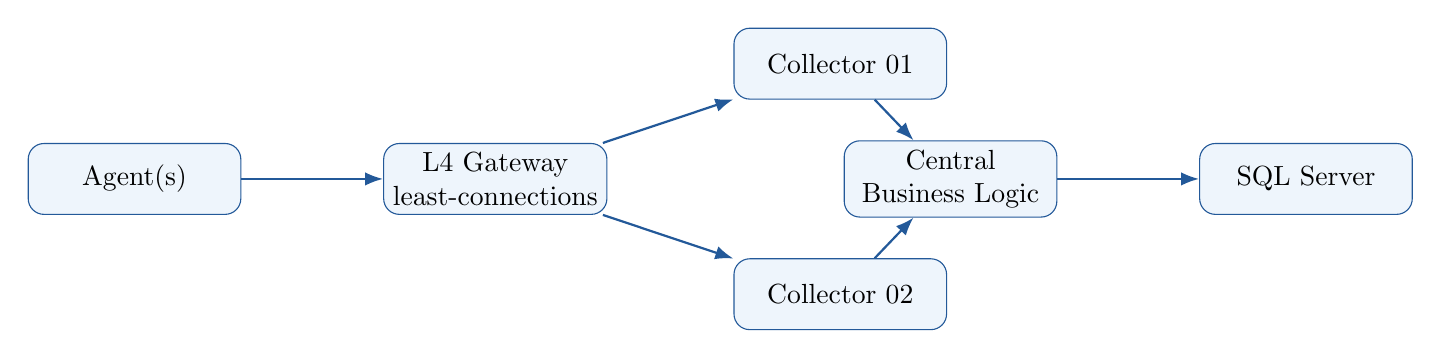
\begin{tikzpicture}[
  node distance=1.4cm and 1.8cm,
  box/.style={draw=lgblue, rounded corners=2mm, fill=lglight, minimum width=2.7cm, minimum height=0.9cm, align=center},
  arr/.style={-{Latex[length=2.3mm]}, thick, draw=lgblue}
]
\node[box] (agents) {Agent(s)};
\node[box, right=of agents] (gw) {L4 Gateway\\least-connections};
\node[box, above right=0.55cm and 1.6cm of gw] (c1) {Collector 01};
\node[box, below right=0.55cm and 1.6cm of gw] (c2) {Collector 02};
\node[box, right=3.0cm of gw] (central) {Central\\Business Logic};
\node[box, right=of central] (sql) {SQL Server};
\draw[arr] (agents) -- (gw);
\draw[arr] (gw) -- (c1);
\draw[arr] (gw) -- (c2);
\draw[arr] (c1) -- (central);
\draw[arr] (c2) -- (central);
\draw[arr] (central) -- (sql);
\end{tikzpicture}%
}
\caption{Kiến trúc P1: Gateway + hai Collector, trong khi Central vẫn giữ nghiệp vụ.}
\label{fig:p1-architecture}
\end{figure}

Gateway chỉ làm nhiệm vụ chuyển tiếp byte (byte relay) và chọn Collector theo thuật toán ít kết nối nhất (\textit{least-connections}) kết hợp kiểm tra sức khỏe tương tự cơ chế cân bằng tải TCP L4 trong thực tế \cite{nginx_tcp_lb}. Trong phân công P1, Sinh viên C phát triển một ứng dụng Collector dùng chung; khi kiểm thử và triển khai, hai node Collector 01 và Collector 02 là hai instance của cùng một Collector binary (chạy độc lập với cấu hình port hoặc máy khác nhau), bảo đảm không bị lệch giao thức. Mỗi Collector có đầy đủ parser, xác thực, hàng đợi và socket thật. Collector liên tục báo trạng thái sẵn sàng (readiness); Gateway không điều phối kết nối mới tới các node không khỏe mạnh. Blueprint không yêu cầu di chuyển socket đang mở hoặc chuyển đổi dự phòng không gián đoạn; nếu Collector gặp sự cố, Agent được phép ngắt kết nối và tự động kết nối lại sang node khác (thời gian failover p95 $\le 45$ giây là mục tiêu thiết kế [DESIGN TARGET]).

\begin{beginnerbox}
\textbf{Readiness} trả lời ``node hiện có sẵn sàng nhận kết nối mới không?''; \textbf{failover} là chuyển sang node khác khi node hiện tại lỗi; \textbf{fencing} là ngăn node cũ/stale tiếp tục hành xử như nó còn quyền sau một thay đổi phiên/thế hệ. Đây là các khái niệm P1, không cần dùng để hiểu MVP ban đầu.
\end{beginnerbox}

\subsection{Nội dung 10: Thực nghiệm và đánh giá}

Kế hoạch nguồn nêu 33 scenario, bao gồm unit/integration/failure/load. Các nhóm kiểm thử cần có:
\begin{itemize}
    \item parser: partial reads, nhiều frame dính nhau, length sai, frame quá lớn;
    \item rule/Incident: streak, hysteresis, dedup, recovery, relapse, hai Admin conflict;
    \item Agent/Server: disconnect, reconnect, duplicate batch, malformed message;
    \item persistence: restart Central, DB degraded, restore và crash consistency;
    \item multi-client: 10/20/50 simulated Agent, 2 Admin realtime;
    \item P1: routing/readiness/collector kill/failover nếu được triển khai;
    \item deployment: localhost, LAN trên máy thật và bằng chứng Internet nếu hạ tầng cho phép.
\end{itemize}

Chỉ được báo cáo kết quả hiệu năng khi test thật có raw CSV/run configuration. Các con số trong blueprint là \textbf{target}, không được trình bày như kết quả thực nghiệm.

\subsubsection{Giới hạn của đề tài}

\begin{itemize}
    \item MVP chỉ một tổ chức và một lab mặc định; không multi-tenancy phức tạp.
    \item Không remote desktop, remote shell, thao tác hệ điều hành tùy ý hoặc restart service từ xa.
    \item Không Kubernetes, Redis/Kafka hoặc distributed framework nặng chỉ để tăng số công nghệ.
    \item Không AI/anomaly detection trong cam kết 5 tuần.
    \item P1 Gateway + 2 Collector là tùy điều kiện; nếu M4 chưa đạt hoặc còn lỗi nghiêm trọng thì phải DEFER.
    \item Internet live phụ thuộc NAT/CGNAT (RFC 6598 \cite{rfc6598})/firewall/hạ tầng. Nếu không thể demo live, cần mô tả topology trung thực và có bằng chứng thay thế phù hợp yêu cầu môn.
    \item Rubric/checklist chính thức của lớp chưa được xác minh trong Master Plan nguồn; vì vậy tài liệu này không cam kết điểm số.
\end{itemize}

\subsection{Bảng truy vết yêu cầu cốt lõi}

\begin{table}[!ht]
\centering
\caption{Functional Requirements được bảo toàn từ Master Plan.}
\label{tab:fr-trace}
\scriptsize
\begin{tabularx}{\textwidth}{p{1.1cm} p{3.1cm} X >{\raggedright\arraybackslash}p{2.6cm}}
\toprule
\textbf{FR} & \textbf{Chức năng} & \textbf{Acceptance ở mức thiết kế} & \textbf{Task/Test} \\
\midrule
FR01 & Auth/enrollment & Token bind DeviceId; invitation một lần & A004/B004/C003; T13--T15 \\
FR02 & Telemetry & CPU host, RAM physical, NIC, uptime; error=null & A005/A006; T07/T18 \\
FR03 & Service check & Local TCP allowlist $\leq 5$, timeout 2s & A007; T06/T18 \\
FR04 & Multi-client & Socket riêng; parser có boundary/bounds & A002/A003/\-B003/A008; T01--T05/T28 \\
FR05 & Detection & 4 rule; streak/hysteresis; một active ticket/key & B005--B008; T06--T10 \\
FR06 & Collaboration & Command phân quyền, version, history & B009/C008/C009; T11--T13 \\
FR07 & Realtime & Snapshot+delta, version merge, slow-client isolation & C005/C006/C016; T16--T17 \\
FR08 & History/report & Paging, bounded query, CSV cơ bản & B011/C010; T21/T30 \\
FR09 & Recovery & Retry/dedup, restart grace, DB degraded & A009/B010; T10/T19--T20 \\
FR10 & Deployment & 2 máy thật, simulator, LAN/Internet proof & A012/A016/\-A018/A019; T31--T33 \\
FR11 & Security & TLS, KDF, role, limits, no secrets & A004/B004/\-C002/C009; T03--T04/T13--T15 \\
FR12 & P1 & 2 Collector instance cùng binary, routing/health/failover & A013--A015/\-B013--B015/\-C013--C015; T23--T27 \\
\bottomrule
\end{tabularx}
\end{table}


\section{Kế hoạch thực hiện:}
\label{sec:ke-hoach}
% ============================================================
% 5. KẾ HOẠCH THỰC HIỆN
% ============================================================

\subsection*{1. Nguyên tắc phân công nhóm 3 người}

Ba thành viên được chia ownership sao cho mỗi người đều có networking/backend thật để phục vụ cả triển khai lẫn vấn đáp cá nhân. Không có vai trò ``chỉ làm UI''.

\begin{table}[!ht]
\centering
\caption{Ma trận phân bổ ngân sách giờ kỹ thuật chi tiết theo 3 Lane (ADR-007).}
\label{tab:workload}
\scriptsize
\begin{tabularx}{\textwidth}{p{0.6cm} X c c c c c c c c}
\toprule
\textbf{Lane} & \textbf{Ownership chính} & \textbf{P0 Core} & \textbf{Harness} & \textbf{Integ.} & \textbf{Viva} & \textbf{P1} & \textbf{Buffer} & \textbf{Tổng} & \textbf{Giờ/tuần} \\
\midrule
A & Agent / Simulator / Load / Gateway & 24.0 h & 10.0 h & 6.0 h & 5.0 h & 15.0 h & 9.0 h & 69.0 h & 13.8 h/t \\
B & Central / SQL / Rule / Auth / Fanout & 27.0 h & 9.0 h & 6.0 h & 5.0 h & 16.0 h & 9.0 h & 72.0 h & 14.4 h/t \\
C & Admin WinForms / Cache / Multi-Admin & 25.5 h & 9.0 h & 6.0 h & 5.0 h & 16.0 h & 9.0 h & 70.5 h & 14.1 h/t \\
\midrule
\multicolumn{2}{l}{\textbf{Tổng cộng toàn dự án (5 tuần)}} & \textbf{76.5 h} & \textbf{28.0 h} & \textbf{18.0 h} & \textbf{15.0 h} & \textbf{47.0 h} & \textbf{27.0 h} & \textbf{211.5 h} & \textbf{42.3 h/t} \\
\bottomrule
\end{tabularx}
\end{table}

Tổng ngân sách kỹ thuật toàn dự án là 211.5 giờ. Kế hoạch đầy đủ này chỉ phù hợp khi nhóm duy trì khoảng 14--15 giờ/người/tuần (thành viên A: 13.8 h/tuần, B: 14.4 h/tuần, C: 14.1 h/tuần; định nghĩa 1 ngày tập trung = 3 giờ kỹ thuật). So với ước tính sơ bộ ~135 giờ của Master Plan nguồn (vốn chỉ tính code tính năng), mức tăng thêm là hoàn toàn minh bạch do bổ sung: 3 bộ test harness độc lập (28.0 h), tích hợp kiểm thử dồn dập (18.0 h), diễn tập vấn đáp kỹ thuật (15.0 h) và dự phòng rủi ro gỡ lỗi (27.0 h).

\textbf{Phương án 12 giờ/người/tuần (Năng lực trần 180 giờ):} Nếu nhóm duy trì định mức 12 giờ/người/tuần ($3 \times 12 \times 5 = 180.0\text{ giờ}$), đồ án chủ động kích hoạt cơ chế DEFER toàn bộ P1 ($-47.0\text{ giờ}$). Khi đó khối lượng công việc cam kết thực tế giảm xuống còn $211.5 - 47.0 = 164.5\text{ giờ}$ (thành viên A: $69.0 - 15.0 = 54.0\text{ giờ}$; B: $72.0 - 16.0 = 56.0\text{ giờ}$; C: $70.5 - 16.0 = 54.5\text{ giờ}$). Khối lượng 164.5 giờ này đã bao gồm đủ $27.0\text{ giờ}$ dự phòng (buffer) cho các thành viên. Khoảng chênh lệch $180.0 - 164.5 = 15.5\text{ giờ}$ đóng vai trò là dung lượng năng lực dự phòng ngoài cam kết (\textit{capacity headroom}), không bị tính dồn vào khối lượng cam kết và không tính trùng với 27 giờ buffer. Mô hình phân công đảm bảo mỗi người có một lane P0 độc lập; P1 bổ sung extension component theo đúng ownership đã chốt.

\begin{warningbox}
Nếu thực tế mỗi người chỉ có khoảng 8 giờ/tuần, tổng 5 tuần chỉ khoảng 120 giờ và còn thiếu buffer học/debug. Khi đó phải chuyển sang 6 tuần hoặc cắt P1/giảm phụ. Không được dùng AI như lý do để giả định thời gian học bằng 0.
\end{warningbox}

\subsection*{2. Kế hoạch theo tuần}

\subsubsection*{Tuần 1 -- Contract, DB, TLS/auth và heartbeat một Agent}

\begin{itemize}
    \item \textbf{A}: A001--A006: wire contract/fixtures; FrameCodec + partial reads; Agent TCP connection + writer queue; TLS client + token enroll; CPU/RAM/NIC/uptime; heartbeat + batch sender.
    \item \textbf{B}: B001--B004: schema migration/seed; repository + transaction boundary; Central TLS accept + bounded ingress; session registry + server auth \& PBKDF2.
    \item \textbf{C}: C001--C004: UI shell + navigation; Admin TCP/TLS RPC client; login/signup WinForms UI; request/response correlation + timeout.
\end{itemize}

\textbf{Checkpoint:} M0/M1 transport: parser fixtures, migration, TLS/auth, heartbeat. M1 đạt được khi luồng mỏng (Thin Vertical Slice) thành công: 1 metric thật từ Agent $\rightarrow$ Central $\rightarrow$ CSDL SQL $\rightarrow$ Admin query hiển thị.

\subsubsection*{Tuần 2 -- Multi-Agent ingest, rule và subscription}

\begin{itemize}
    \item \textbf{A}: A007--A010: service TCP probe; simulator 10/20/50 socket; reconnect/backoff + metric replay; failure injection + counters.
    \item \textbf{B}: B005--B008: ingest + dedup (DeviceId+BootId+BatchId) + commit ACK; liveness monotonic deadline; rule hysteresis/streak; Incident persistence + unique active.
    \item \textbf{C}: C005--C007: bộ nhận snapshot + khởi tạo cache; đồng bộ delta event + điều phối UI thread (\texttt{Invoke}); Dashboard + Lab View + Device Detail.
\end{itemize}

\textbf{Checkpoint:} M2: 20 simulated Agent chạy 30 phút không crash; parser/dedup/rule/bounds pass; create/recovery + snapshot chạy được.

\subsubsection*{Tuần 3 -- Incident collaboration, history, retention và MVP gate}

\begin{itemize}
    \item \textbf{A}: A011--A012: log xoay vòng, evidence LAN; kiểm thử Agent end-to-end trên hai máy thật.
    \item \textbf{B}: B009--B012: xử lý command (ACK, START, RESOLVE) với OCC; lỗi restart/DB, health, retention và gate M4.
    \item \textbf{C}: C008--C012: Incident list/detail và action binding; RBAC UI, session lifecycle; History/Report/Health views; MVP UI integration; review và quyết định P1 GO/DEFER.
\end{itemize}

\textbf{Checkpoint:} M3/M4: 2 Admin conflict được xử lý; workflow đủ; history/role/restart/retention pass. P0 freeze cuối tuần 3.

\subsubsection*{Tuần 4 -- P1 có điều kiện hoặc ổn định core}

Nếu M4 không đạt, tuần 4 chỉ sửa core. Nếu M4 đạt và không còn lỗi nghiêm trọng:
\begin{itemize}
    \item \textbf{A}: A013--A014: Gateway least-connections admission; duplex relay và health polling.
    \item \textbf{B}: B013--B017: internal Collector listener/dispatch; session generation across Collector; loss recovery/offline suppression; tune SQL/index/ingest budget; regression parser/auth/incident.
    \item \textbf{C}: C013--C016: ứng dụng Collector dùng chung (cho 2 instance); upstream multiplex, reply router; readiness và bounded buffer; kiểm thử lỗi đa Admin.
\end{itemize}

\textbf{Checkpoint:} readiness/routing/fencing pass. Kill/failover có thể kéo sang đầu tuần 5; nếu prerequisite trễ thì cắt P1.

\subsubsection*{Tuần 5 -- Freeze, regression, proof, release và viva}

\begin{itemize}
    \item \textbf{A}: A015--A020: tích hợp LB, collector kill, Internet deploy/fallback; load/reconnect storm; proof, release scripts và viva A.
    \item \textbf{B}: B018--B020: khôi phục DB và chứng minh crash consistency; audit tài liệu hệ thống; viva B và backup handover.
    \item \textbf{C}: C017--C020: kiểm thử hồi quy UI, settings cleanup; diễn tập demo, chuẩn bị backup; release checklist, README và viva C.
\end{itemize}

\textbf{Freeze rule:} giữa tuần 5 ngừng thêm feature; chỉ sửa lỗi critical có regression test. Chốt video/config/commit/package cùng phiên bản.

\subsection*{3. Gantt chart 5 tuần theo phong cách đề cương}

\hspace*{-0.8cm}
\resizebox{\textwidth}{!}{
\begin{ganttchart}[
    x unit=1.35cm,
    y unit chart=0.62cm,
    canvas/.append style={fill=none, draw=black!5, line width=1pt},
    hgrid style/.style={draw=black!8, line width=.7pt},
    vgrid={*1{draw=black!8, line width=.7pt}},
    title/.style={draw=none, fill=none},
    title label font=\bfseries,
    bar label font=\small\color{black!75},
    bar label node/.append style={text width=8.5cm, align=left},
    bar/.append style={draw=none, fill=primaryblue},
    group/.append style={fill=secondarygreen},
    group label node/.append style={text width=8.5cm, align=left, font=\bfseries},
    milestone/.append style={fill=criticalred, draw=criticalred},
    milestone label font=\small\itshape
]{1}{5}
\gantttitlelist{1,...,5}{1}\\
\ganttgroup{P0 -- MVP}{1}{3}\\
\ganttbar{Contract, protocol, TLS/auth, DB skeleton}{1}{1}\\
\ganttbar{Multi-Agent ingest, liveness, rule engine}{2}{2}\\
\ganttbar{Incident collaboration, history, LAN MVP}{3}{3}\\
\ganttgroup{P1 -- chỉ khi M4 đạt}{4}{5}\\
\ganttbar{Gateway + 2 Collector + readiness/routing}{4}{4}\\
\ganttbar{Kill/failover/load test và release proof}{5}{5}\\
\ganttgroup{Release + Viva}{1}{5}\\
\ganttbar{Recall/viva hằng ngày + review cuối tuần}{1}{5}\\
\ganttmilestone{M0 Architecture Frozen}{1}\\
\ganttmilestone{M2 Multi-Agent Stable}{2}\\
\ganttmilestone{M4 Product MVP / P1 Gate}{3}\\
\ganttmilestone{M5 High-score Networking (nếu pass)}{4}\\
\ganttmilestone{M6/M7 Release + Viva Ready}{5}
\end{ganttchart}
}

\subsection*{4. Milestones và exit criteria}

\begin{table}[!ht]
\centering
\caption{Milestone chính của dự án.}
\label{tab:milestones}
\small
\begin{tabularx}{\textwidth}{p{1cm} p{3.8cm} p{2.2cm} X}
\toprule
\textbf{M} & \textbf{Mục tiêu} & \textbf{Thời điểm} & \textbf{Exit criteria} \\
\midrule
M0 & Architecture Frozen & Đầu W1 & Nhóm review contract/schema/owner; môi trường 3 máy; blocker được ghi rõ \\
M1 & Single Agent End-to-End & Cuối W1--đầu W2 & TLS/auth/HB/metric $\rightarrow$ Central $\rightarrow$ DB $\rightarrow$ Admin query \\
M2 & Multi-Agent Stable & Cuối W2 & 20 sim/30 phút, 0 crash, parser/dedup/rule/bounds pass \\
M3 & Incident Workflow Complete & W3 & ACK/assign/start/recover/resolve + history; 2 Admin conflict \\
M4 & Product MVP & Cuối W3 & P0 flow 2 máy thật, roles/TLS/restart/retention/UI, không còn Sev1/2 \\
M5 & High-score Networking & Cuối W4--đầu W5 nếu làm & 2 Collector thật, selection/readiness/fencing/kill-failover proof \\
M6 & Release Candidate & W5 & Actual tests, restore, clean-machine package, README, known issues, freeze \\
M7 & Viva Ready & Cuối W5 & 3 người trả lời/live-code/debug phần mình; 2 dry-run demo \\
\bottomrule
\end{tabularx}
\end{table}

\subsection*{5. Dependency graph}

\begin{figure}[!ht]
\centering
\begin{tikzpicture}[
  node distance=1.15cm and 1.25cm,
  box/.style={draw=lgblue, rounded corners=2mm, fill=lglight, minimum width=3.1cm, minimum height=0.85cm, align=center},
  arr/.style={-{Latex[length=2.3mm]}, thick, draw=lgblue}
]
\node[box] (contract) {Contract + schema};
\node[box, below left=of contract] (agent) {Agent transport};
\node[box, below=of contract] (central) {Central pipeline};
\node[box, below right=of contract] (admin) {Admin RPC + auth};
\node[box, below=1.4cm of central] (ingest) {Ingest + rule};
\node[box, below right=1.2cm and -0.2cm of ingest] (incident) {Incident collaboration};
\node[box, below=of incident] (mvp) {MVP gate};
\node[box, below left=of mvp] (p1) {P1 tùy chọn};
\node[box, below=of mvp] (release) {Release};
\node[box, below right=of mvp] (viva) {Viva};
\draw[arr] (contract) -- (agent);
\draw[arr] (contract) -- (central);
\draw[arr] (contract) -- (admin);
\draw[arr] (agent) -- (ingest);
\draw[arr] (central) -- (ingest);
\draw[arr] (ingest) -- (incident);
\draw[arr] (admin) -- (incident);
\draw[arr] (incident) -- (mvp);
\draw[arr] (mvp) -- (p1);
\draw[arr] (mvp) -- (release);
\draw[arr] (p1) -- (release);
\draw[arr] (release) -- (viva);
\end{tikzpicture}
\caption{Quan hệ phụ thuộc ở mức cao.}
\label{fig:dependency}
\end{figure}

Chuỗi nhạy tiến độ trong blueprint là C008 $\rightarrow$ B009 $\rightarrow$ B010/B011 $\rightarrow$ C011 $\rightarrow$ M4 rồi mới đến Collector/Gateway. UI sử dụng DTO fixtures/mock để không phải chờ toàn bộ server hoàn thành.

Trong trường hợp gate M4 quyết định hoãn (DEFER) P1 để tập trung tối đa cho độ ổn định MVP, đồ án áp dụng quy tắc tách rời phụ thuộc (DAG Decoupling): LG-A-016 (Rehearsal/Load) phụ thuộc trực tiếp vào LG-A-012 (MVP proof) thay vì LG-A-015; LG-B-016 (SQL Tuning) phụ thuộc vào LG-B-012 (Incident Acceptance) thay vì LG-B-015; LG-C-016 (Multi-Admin Concurrency) phụ thuộc vào LG-C-011 (MVP UI) thay vì LG-C-015. Nhờ vậy, dependency graph tách P0 khỏi P1 để việc trì hoãn nhánh P1 không chặn đường hoàn thành MVP.

\subsection*{6. Quy tắc co giãn lịch}

\begin{table}[!ht]
\centering
\caption{Phương án co giãn scope theo thời gian thực tế.}
\small
\begin{tabularx}{\textwidth}{p{2cm} X}
\toprule
\textbf{Thời lượng} & \textbf{Quyết định} \\
\midrule
3 tuần & 1 lab, 1 server, 2 máy thật + 10 sim, 4 rule, Incident + auth/TLS; cắt P1/P2/P3, giảm polish nhưng không bỏ test core \\
4 tuần & Bỏ 9 task P1; tập trung MVP + viva; UI dùng mock sớm; giữ kiểm tra khả thi Internet \\
5 tuần & Baseline có điều kiện 12--15 giờ/người/tuần; M4 cuối W3; P1 chỉ khi gate pass \\
6 tuần & W4 ổn định core; W5 P1; W6 release/viva, soak/restore/failure test; không tự thêm AI \\
\bottomrule
\end{tabularx}
\end{table}

\textbf{P1 cutoff:} nếu cuối W3 chưa đạt M4, còn Sev1/2 hoặc không còn khoảng 9 giờ/người ngoài reserve, 9 task P1 phải DEFER. Các test P1 ghi SKIPPED, M5 ghi DEFERRED thay vì giả vờ DONE.

\subsection*{7. Kế hoạch kiểm thử}

Kế hoạch nguồn có 33 scenario thiết kế. Tài liệu này nhóm lại thành các tầng:
\begin{enumerate}
    \item \textbf{Unit}: FrameCodec/parser, rule threshold/hysteresis, state transition, LB selection.
    \item \textbf{Integration}: Agent$\leftrightarrow$Central, Admin$\leftrightarrow$Central, SQL persistence, auth/TLS.
    \item \textbf{Failure}: kill Agent, disconnect mạng, malformed/duplicate packet, restart Central, DB degraded, reconnect storm.
    \item \textbf{Load}: 10/20/50 simulated Agents; theo dõi crash, queue/drop, latency và resource.
    \item \textbf{Deployment}: localhost chỉ dùng khi dev; bằng chứng chính phải có LAN trên máy thật; Internet proof tùy hạ tầng.
\end{enumerate}

\begin{beginnerbox}
Mỗi test nên có bốn dòng cố định: \textbf{Setup} (chuẩn bị gì), \textbf{Action} (làm gì), \textbf{Expected} (đúng phải ra sao), \textbf{Evidence} (log/screenshot/CSV nào chứng minh). Cách này giúp demo và vấn đáp không dựa vào ``em nhớ là nó chạy''.
\end{beginnerbox}

\subsection*{8. Demo cuối kỳ dự kiến}

Kịch bản nguồn khoảng 7 phút 45 giây:
\begin{enumerate}
    \item Login và mở Lab View.
    \item Chứng minh 2 máy thật + một số simulated Agent đang online.
    \item Kill một Agent thật $\rightarrow$ offline Incident.
    \item Admin ACK/START.
    \item Agent reconnect $\rightarrow$ RECOVERED $\rightarrow$ RESOLVED.
    \item Tạo \texttt{SERVICE\_DOWN} và chứng minh rule không spam.
    \item Mở Admin thứ hai, chứng minh realtime/xung đột quyền.
    \item Nếu P1 pass: hiển thị 2 Collector, LB và collector kill.
    \item Chứng minh LAN/Internet theo topology thật; nếu Internet live lỗi thì dùng phương án backup đã chuẩn bị.
    \item Kết thúc bằng test evidence và ownership của từng thành viên.
\end{enumerate}

\subsection*{9. Vấn đáp cá nhân và Definition of Done}

Mỗi thành viên có 20 task card và 30 câu hỏi vấn đáp trong blueprint gốc. Một task chỉ được coi là DONE khi: code chạy; edge case chính được xử lý; exception/logging hợp lý; test có ý nghĩa; tài liệu cập nhật; PR được review; flow networking chạy LAN nếu liên quan; owner giải thích được API/flow/failure và vượt viva tương ứng.

\begin{vivabox}
Quy tắc bắt buộc với code có AI hỗ trợ: owner phải chỉ được đoạn code nằm ở file/class nào, input/output là gì, failure path là gì, test nào chứng minh, và vì sao chọn API đó. ``AI viết cho em'' không phải câu trả lời chấp nhận được trong vấn đáp.
\end{vivabox}

\subsection*{10. Git workflow và release checklist}

\begin{itemize}
    \item \texttt{main} luôn build/test; không cần branch \texttt{develop} cho nhóm 3 nếu quy trình PR đủ rõ.
    \item Branch theo task: \texttt{feature/LG-A-002-frame-codec}, \texttt{fix/LG-B-009-ack-conflict}.
    \item Mỗi task có issue + branch + PR nhỏ + ít nhất một review khác owner.
    \item Thay đổi Shared.Protocol cần cả nhóm review.
    \item Không force-push \texttt{main}; không commit password/certificate private key/DB secret.
    \item Commit convention: \texttt{feat(protocol)}, \texttt{fix(incident)}, \texttt{test(parser)}, \texttt{docs(viva)}.
    \item Môi trường thực thi: Chuẩn hóa trên .NET 9.0 SDK (baseline của dự án hiện được kiểm thử trên môi trường phát triển của nhóm; tính tương thích phòng máy UIT cần được xác thực trước khi triển khai thực tế \cite{mslearn_dotnet_support}); khuyến nghị nâng cấp sang .NET 10 LTS sau khi đối soát trên máy trạm đích.
\end{itemize}

Trước release: không còn Sev1/2; restore/retention/bounded queue được kiểm tra; TLS/auth/role negative test pass; LAN proof có 2 máy thật; số simulated client được ghi rõ; P1 chỉ được claim nếu routing/kill/fencing pass; package/config/cert/migration/runbook/README đủ cho máy sạch; video/config/tag/checksum cùng commit; ba owner tự demo và vấn đáp phần mình.


\section{Phụ lục A -- Bảng thuật ngữ nhập môn:}
% ============================================================
% PHỤ LỤC A - GLOSSARY
% ============================================================

Phụ lục này được thêm để người mới không phải đoán nghĩa các từ tiếng Anh xuất hiện trong Master Plan.

\begin{longtable}{p{3.4cm} p{11.2cm}}
\toprule
\textbf{Thuật ngữ} & \textbf{Giải thích trong ngữ cảnh LabGuard} \\
\midrule
\endfirsthead
\toprule
\textbf{Thuật ngữ} & \textbf{Giải thích trong ngữ cảnh LabGuard} \\
\midrule
\endhead
Agent & Chương trình chạy trên máy cần giám sát. Nó thu trạng thái máy, gửi heartbeat/telemetry và reconnect khi cần. Không phải AI Agent. \\
Telemetry & Dữ liệu trạng thái được gửi từ xa: CPU, RAM, NIC, uptime, service status. \\
Heartbeat (HB) & Gói nhỏ gửi định kỳ để chứng minh Agent vẫn còn sống ở tầng ứng dụng. \\
Liveness & Câu hỏi ``thành phần này còn đang hoạt động không?''; thường được quyết định từ heartbeat + timeout/deadline. \\
Central Server & Máy chủ giữ nghiệp vụ chính: device state, rule, Incident, DB và realtime cho Admin. \\
Incident & Phiếu sự cố có vòng đời từ phát hiện đến xử lý xong; không đồng nghĩa một dòng log. \\
ACK / Acknowledge & Xác nhận đã nhận sự cố hoặc đã nhận message, tùy ngữ cảnh protocol/Incident. \\
TCP & Giao thức hướng kết nối cung cấp byte stream tin cậy, có thứ tự; không giữ biên message của ứng dụng. \\
Byte stream & TCP đưa ra chuỗi byte liên tục; một lần đọc có thể trả một phần message hoặc nhiều message dính nhau. \\
Framing & Quy tắc để receiver biết message bắt đầu/kết thúc ở đâu trên byte stream. \\
Length-prefix & Cách framing: gửi độ dài trước, rồi gửi đúng số byte payload. LabGuard dự kiến dùng 4 byte length. \\
Partial read & Một lần ReadAsync nhận ít byte hơn số byte của message; code phải đọc tiếp cho đủ. \\
Big-endian & Quy ước đặt byte có trọng số lớn trước khi biểu diễn số nhiều byte trên wire. \\
JSON / UTF-8 & Định dạng dữ liệu text và encoding dự kiến cho payload của protocol. \\
Envelope & Lớp bọc chung của message gồm version, messageType, requestId, deviceId, sentAtUtc và payload. \\
RequestId / CommandId & Mã định danh yêu cầu/lệnh để trace, retry và phát hiện trùng. \\
Deduplication & Loại bỏ việc xử lý lại một dữ liệu/lệnh đã commit trước đó. \\
Idempotency & Tính chất cho phép retry mà kết quả cuối không bị nhân đôi ngoài ý muốn. \\
Queue & Hàng đợi công việc/message giữa producer và consumer. \\
Bounded queue & Queue có giới hạn; khi đầy phải chờ/drop/fail theo policy thay vì ăn RAM vô hạn. \\
Backpressure & Cơ chế làm phía gửi chậm lại khi phía nhận không xử lý kịp. \\
Backoff & Sau lỗi kết nối, chờ một khoảng tăng dần trước khi thử lại để tránh reconnect storm. \\
Reconnect storm & Nhiều client reconnect đồng loạt, tạo tải đột biến cho server. \\
Rule engine & Khối đánh giá telemetry để quyết định có bất thường hay không. \\
Streak & Số mẫu liên tiếp cùng vi phạm; dùng để tránh phản ứng với một spike đơn lẻ. \\
Hysteresis & Dùng ngưỡng mở và ngưỡng hồi phục khác nhau để tránh trạng thái bật/tắt liên tục gần threshold. \\
ConditionState & Trạng thái kỹ thuật của điều kiện lỗi (ACTIVE/RECOVERED/UNKNOWN), tách khỏi workflow xử lý của con người. \\
Race condition & Kết quả sai/không ổn định do nhiều thao tác concurrent cùng đọc/ghi state. \\
Transaction & Nhóm thao tác DB được coi như một đơn vị nguyên tử: hoặc commit đủ, hoặc rollback. \\
rowversion & Datatype riêng của SQL Server (8 byte, do CSDL tự sinh khi row được insert/update; binary(8) thông thường không có semantics tự cập nhật này; không phải date/time); dùng làm token OCC. \\
UI Marshal & Chuyển giao dữ liệu từ luồng nền/mạng về luồng giao diện qua \texttt{Control.Invoke}, \texttt{BeginInvoke} hoặc \texttt{InvokeAsync} để bảo đảm an toàn đa luồng trên WinForms. \\
Snapshot & Ảnh trạng thái đầy đủ tại một thời điểm. \\
Delta / Event & Chỉ phần thay đổi sau snapshot; dùng để update realtime tiết kiệm hơn. \\
Slow-client isolation & Không để một Admin nhận dữ liệu chậm làm block mọi subscriber khác. \\
TLS & Lớp bảo vệ kênh truyền: mã hóa + xác thực endpoint theo certificate/config. \\
Certificate & Chứng thư số dùng trong TLS để xác nhận identity của endpoint và thiết lập kênh bảo mật. \\
Hashing mật khẩu & Biến password thành giá trị một chiều để server không lưu password gốc. \\
Salt & Dữ liệu ngẫu nhiên thêm vào password trước KDF để chống precomputed hash/rainbow table. \\
KDF & Password Key Derivation Function; cố tình tốn tính toán hơn hash nhanh để tăng chi phí brute force. \\
Authentication & Xác định ``ai đang kết nối''. \\
Authorization & Xác định identity đó được phép thao tác gì. \\
RBAC & Role-Based Access Control; phân quyền dựa trên 3 vai trò: Admin (toàn quyền, phân công, quản trị), Operator (xử lý sự cố: ACK/START/RESOLVE), Viewer (chỉ đọc). \\
Retention & Quy định dữ liệu giữ bao lâu trước khi aggregate/purge. \\
Purge & Xóa dữ liệu cũ theo retention policy. \\
Gateway & Điểm vào đứng trước nhiều Collector; ở P1 chọn node và relay kết nối. \\
Collector & Server Agent-facing ở P1, nhận/parse/auth/queue rồi chuyển dữ liệu lên Central. \\
Load balancing (LB) & Phân phối kết nối mới giữa nhiều server để tránh một node ôm hết tải. \\
Least connections & Chọn server đang có ít connection active hơn. \\
Health check & Kiểm tra node còn hoạt động và phản hồi đúng không. \\
Readiness & Cho biết node có sẵn sàng nhận công việc/kết nối mới không. \\
Failover & Khi node lỗi, client/workload chuyển sang node khác. Blueprint chấp nhận có gián đoạn. \\
Fencing & Ngăn session/node cũ tiếp tục ghi dữ liệu như thể nó vẫn còn quyền sau reconnect/failover. \\
Session generation & Số thế hệ của phiên; phiên reconnect mới phải mới hơn để loại update từ phiên cũ. \\
DAG & Directed Acyclic Graph; đồ thị phụ thuộc task không có vòng lặp. \\
WIP & Work In Progress; giới hạn số việc một người đang làm cùng lúc để tránh mở quá nhiều task. \\
MVP & Phiên bản nhỏ nhất nhưng hoàn chỉnh end-to-end, có giá trị demo và test thật. \\
P0/P1/P2/P3 & Mức ưu tiên: bắt buộc / nâng cao / stretch / tương lai. \\
Definition of Done & Điều kiện để task thực sự DONE: code + test + docs + review + owner hiểu và vấn đáp được. \\
Regression test & Test chạy lại để chứng minh sửa một lỗi/tính năng không làm hỏng hành vi đã đúng trước đó. \\
Failure injection & Chủ động tạo lỗi như disconnect/service down để kiểm tra hệ thống xử lý đúng. \\
Simulator & Chương trình tạo nhiều Agent/socket giả lập về thiết bị nhưng kết nối mạng và protocol là thật. \\
CGNAT & Cơ chế NAT của nhà mạng khiến thiết bị không có public IPv4 riêng, có thể làm inbound Internet khó/không khả thi. \\
\bottomrule
\end{longtable}


\section{Phụ lục B -- Danh mục 60 công việc theo người phụ trách:}
% ============================================================
% PHỤ LỤC B - 60 TASK MAP
% Các tên task được đồng bộ từ tài liệu WBS chi tiết (WBS_TASKS.csv).
% ============================================================

Bảng dưới đây là bản rút gọn 4 cột trích xuất từ Master WBS CSV (\texttt{WBS\_TASKS.csv}, tệp master có ít nhất 27 cột với đầy đủ thông tin owner, hours, category, prerequisites, verification, failure mode và viva evidence). Việc duy trì 60 task (20 task/người) là kết quả tự nhiên sau khi tái phân bổ công việc nhằm đảm bảo tính độc lập và cân bằng khối lượng kỹ thuật giữa 3 làn song song. Toàn bộ các task hiện ở trạng thái TODO vì đây là checkpoint thiết kế; việc triển khai MVP bắt đầu theo kế hoạch sau khi contract được freeze.

\begingroup
\scriptsize
\renewcommand{\arraystretch}{0.82}
\setlength{\tabcolsep}{3pt}
\begin{longtable}{p{1.5cm} p{0.9cm} p{10.5cm} p{1.6cm}}
\toprule
\textbf{Task} & \textbf{Tuần} & \textbf{Nội dung tóm tắt từ Master Plan} & \textbf{Priority} \\
\midrule
\endfirsthead
\toprule
\textbf{Task} & \textbf{Tuần} & \textbf{Nội dung tóm tắt từ Master Plan} & \textbf{Priority} \\
\midrule
\endhead
LG-A-001 & W1 & Chốt wire contract và protocol fixtures & P0 \\
LG-A-002 & W1 & FrameCodec và xử lý partial reads / message framing & P0 \\
LG-A-003 & W1 & Agent TCP connection và writer queue & P0 \\
LG-A-004 & W1 & TLS client và local identity/enrollment & P0 \\
LG-A-005 & W1 & Thu CPU, RAM, NIC, uptime & P0 \\
LG-A-006 & W1 & Heartbeat và batch sender & P0 \\
LG-A-007 & W2 & Local TCP service probe theo allowlist & P0 \\
LG-A-008 & W2 & Agent Simulator 10/20/50 socket độc lập & P0 \\
LG-A-009 & W2 & Reconnect backoff và metric replay/retry & P0 \\
LG-A-010 & W2 & Failure injection và counters & P0 \\
LG-A-011 & W3 & Log xoay vòng và evidence hỗ trợ debug & P0 \\
LG-A-012 & W3 & MVP Agent end-to-end trên hai máy thật / LAN & P0 \\
LG-A-013 & W4 & Gateway least-connections admission & P1 \\
LG-A-014 & W4 & Gateway duplex relay và health polling & P1 \\
LG-A-015 & W5 & LB integration và collector kill/failover proof & P1 \\
LG-A-016 & W5 & Internet deployment chuẩn và fallback & P0/Release \\
LG-A-017 & W5 & Load test và reconnect storm & P0/Release \\
LG-A-018 & W5 & Thu proof LAN/Internet cho release candidate & P0/Release \\
LG-A-019 & W5 & Release scripts và package checksum & P0/Release \\
LG-A-020 & W5 & Viva A và bàn giao backup & P0/Viva \\
\midrule
LG-B-001 & W1 & Schema migrations và seed an toàn & P0 \\
LG-B-002 & W1 & SQL repositories và transaction boundary & P0 \\
LG-B-003 & W1 & Central accept TLS và bounded ingress & P0 \\
LG-B-004 & W1 & Session registry, server auth PBKDF2 \& RBAC & P0 \\
LG-B-005 & W2 & Metric ingestion, dedup ProcessedBatches, commit ACK & P0 \\
LG-B-006 & W2 & Liveness registry và monotonic deadline evaluator & P0 \\
LG-B-007 & W2 & Rule evaluator: hysteresis và counters & P0 \\
LG-B-008 & W2 & Incident persistence và unique active constraint & P0 \\
LG-B-009 & W3 & Commands ACK/ASSIGN/START/RESOLVE + rowversion OCC & P0 \\
LG-B-010 & W3 & Restart/DB fault handling và Central health & P0 \\
LG-B-011 & W3 & Retention, query/report và restore plan & P0 \\
LG-B-012 & W3 & MVP concurrency và Incident acceptance & P0 \\
LG-B-013 & W4 & Internal Collector listener và dispatch & P1 \\
LG-B-014 & W4 & Session generation qua Collector & P1 \\
LG-B-015 & W4 & Collector loss recovery và offline suppression & P1 \\
LG-B-016 & W4 & Tune SQL index và ingest budgets & P0/Stability \\
LG-B-017 & W4 & Parser/auth/incident regression & P0/Stability \\
LG-B-018 & W5 & DB restore và crash consistency proof & P0/Release \\
LG-B-019 & W5 & Audit tài liệu architecture/protocol/database & P0/Docs \\
LG-B-020 & W5 & Viva B và bàn giao backup & P0/Viva \\
\midrule
LG-C-001 & W1 & WinForms UI shell wireframe và mock DTO & P0 \\
LG-C-002 & W1 & Admin TCP/TLS RPC client connection & P0 \\
LG-C-003 & W1 & Login/Signup WinForms UI \& token storage client & P0 \\
LG-C-004 & W1 & Khớp cặp Request/Response correlation và timeout & P0 \\
LG-C-005 & W2 & Bộ nhận Snapshot và khởi tạo cache Admin & P0 \\
LG-C-006 & W2 & Admin cache merge, reconnect và UI-thread marshal & P0 \\
LG-C-007 & W2 & Dashboard, Lab View, Device Detail & P0 \\
LG-C-008 & W3 & Incident list/detail và action binding & P0 \\
LG-C-009 & W3 & RBAC UI UX và session lifecycle client-side & P0 \\
LG-C-010 & W3 & History/Report/Health views & P0 \\
LG-C-011 & W3 & MVP UI integration và accessibility & P0 \\
LG-C-012 & W3 & MVP review và P1 GO/DEFER gate & P0/Gate \\
LG-C-013 & W4 & Collector Agent-facing host (binary dùng chung) & P1 \\
LG-C-014 & W4 & Collector upstream multiplex và reply router & P1 \\
LG-C-015 & W4 & Collector readiness/health và bounded buffers & P1 \\
LG-C-016 & W4 & Multi-admin concurrency và race condition tests & P0/Stability \\
LG-C-017 & W5 & UI release regression và settings cleanup & P0/Release \\
LG-C-018 & W5 & Demo rehearsal và backup assets & P0/Demo \\
LG-C-019 & W5 & Release review checklist và README & P0/Release \\
LG-C-020 & W5 & Viva C và bàn giao backup & P0/Viva \\
\bottomrule
\end{longtable}
\endgroup
\normalsize



\section{Phụ lục C -- Khung vấn đáp cá nhân:}
% ============================================================
% PHỤ LỤC C - VIVA FRAMEWORK
% ============================================================

Bộ 3 cẩm nang kèm 90 câu hỏi vấn đáp chi tiết (30 câu/người) được biên soạn và bàn giao tại thư mục \texttt{handbooks/} (gồm \texttt{HANDBOOK\_A.md}, \texttt{HANDBOOK\_B.md}, \texttt{HANDBOOK\_C.md}). Phụ lục này tóm lược các trọng tâm kỹ thuật cốt lõi và ví dụ câu hỏi điển hình của từng thành viên.

\subsection*{Người A -- Agent, Codec, Simulator, Deploy/Gateway}

\textbf{Phải hiểu sâu:} TCP byte stream, framing, partial read, writer queue, SslStream, heartbeat, service probe, reconnect/backoff, retry/dedup ở client, simulator nhiều socket, LAN/Internet topology, least-connections nếu P1.

\begin{vivabox}
Ví dụ câu hỏi cần có trong handbook A:
\begin{enumerate}
    \item Tại sao một lần \texttt{ReadAsync} không thể coi là một message?
    \item Nếu 4 byte length bị chia thành hai lần đọc thì FrameCodec xử lý thế nào?
    \item Tại sao cần giới hạn max frame size?
    \item Heartbeat dùng để giải quyết vấn đề gì mà \texttt{socket.Connected} không đủ?
    \item Backoff giúp tránh reconnect storm ra sao?
    \item Agent Simulator có gì ``thật'' và có gì ``giả''?
    \item Khi Collector chết ở P1, Agent cũ có được migrate socket không? Vì sao blueprint không yêu cầu zero-downtime?
\end{enumerate}
\end{vivabox}

\subsection*{Người B -- Central Server, Database, Rule Engine, Auth Server, Snapshot}

\textbf{Phải hiểu sâu:} accept nhiều client bằng async I/O ThreadPool, session registry, PBKDF2 băm mật khẩu + salt, server-side RBAC, commit ACK, liveness deadline bằng monotonic clock, streak/hysteresis, Incident dual-state, transaction boundary, rowversion OCC, telemetry dedup, retention/restore, internal Collector routing nếu P1.

\begin{vivabox}
Ví dụ câu hỏi cần có trong handbook B:
\begin{enumerate}
    \item Vì sao ACK metrics nên gửi sau một điểm commit xác định?
    \item Hai Admin cùng ACK một Incident tạo race condition như thế nào?
    \item Transaction khác lock trong code ở đâu?
    \item rowversion giúp phát hiện conflict ra sao?
    \item Vì sao cần tách ConditionState khỏi Incident workflow?
    \item Hysteresis khác threshold đơn như thế nào?
    \item Nếu Central restart, dữ liệu nào bắt buộc phải còn và dữ liệu nào có thể mất theo TTL?
\end{enumerate}
\end{vivabox}

\subsection*{Người C -- Admin WinForms, RPC Client, Realtime Cache, Concurrency Test, Collector App}

\textbf{Phải hiểu sâu:} Chu trình WinForms STA, điều phối luồng an toàn (UI marshal bằng \texttt{Invoke}, \texttt{BeginInvoke}, \texttt{InvokeAsync}), đối soát RPC qua \texttt{requestId}, xử lý timeout, đồng bộ cache snapshot/delta, chống race condition khi đa Admin thao tác, cô lập client chậm (\textit{slow-client isolation}) và cấu trúc Collector App (binary P1 dùng chung).

\begin{vivabox}
Ví dụ câu hỏi cần có trong handbook C:
\begin{enumerate}
    \item Authentication và authorization khác nhau thế nào trong LabGuard?
    \item Vì sao ẩn nút trên UI không đủ để bảo vệ quyền RESOLVE?
    \item Snapshot và delta dùng khi nào?
    \item Nếu Admin bị mất một eventSeq rồi reconnect thì phải làm gì?
    \item Vì sao network callback không nên update WinForms control trực tiếp từ background thread?
    \item Slow Admin client có thể ảnh hưởng subscriber khác thế nào và cách cô lập?
    \item Readiness của Collector khác liveness/health check ở điểm nào?
\end{enumerate}
\end{vivabox}

\subsection*{Mẫu trả lời vấn đáp 6 bước}

Khi trả lời một module mình làm, mỗi thành viên nên đi theo thứ tự:
\begin{enumerate}
    \item \textbf{WHAT}: thành phần này là gì?
    \item \textbf{WHY}: nó giải quyết vấn đề gì trong LabGuard?
    \item \textbf{FLOW}: dữ liệu đi từ đâu đến đâu, qua class/API nào?
    \item \textbf{FAILURE}: nếu mạng lỗi/concurrent/invalid input thì sao?
    \item \textbf{VERIFY}: test/log nào chứng minh code hoạt động?
    \item \textbf{TRADE-OFF}: vì sao chọn cách này thay vì cách khác đơn giản/phức tạp hơn?
\end{enumerate}


\section{Tài liệu tham khảo và nguồn thiết kế:}
\begingroup
\small
\setlength{\bibitemsep}{0.6ex}
\nocite{labguard2026,rfc9293,rfc8259,rfc8446,rfc6598,uit_nt106_2022,mslearn_sockets,mslearn_networkstream,mslearn_sslstream,mslearn_winforms_threadsafe,mslearn_channels,mslearn_rowversion,mslearn_sql_express_limits,owasp_password_storage,mslearn_dotnet_support,nginx_tcp_lb}
\justifying\printbibliography[heading=none]
\endgroup

\vspace*{1ex}
\hfill\textit{TP. Hồ Chí Minh, tháng 09 năm 2026}
\nopagebreak\printsignature

\end{document}
